\chapter{Các đa bội \texorpdfstring{\(SU(5)\)}{SU(5)}, các boson chuẩn leptoquark và sự phân rã proton}

\lectureoverview{Thống nhất lớn trở nên cụ thể khi nhóm của Mô hình Chuẩn được nhúng vào \(SU(5)\). Để thấy phát biểu ấy có nghĩa gì, trước hết ta xây dựng lý thuyết biểu diễn cần thiết: biểu diễn cơ bản \(N\), biểu diễn liên hợp của nó \(\overline N\), các tích tensor, các tensor đối xứng và phản đối xứng, và biểu diễn adjoint. Khi đó, một thế hệ của Mô hình Chuẩn được xếp vào tổ hợp gọn đến bất ngờ \(\overline{\mathbf 5}\oplus\mathbf{10}\). Chính đối xứng làm cho cách sắp xếp này đẹp cũng đồng thời đòi hỏi các boson chuẩn mang màu biến quark thành lepton. Sự trao đổi của chúng cho phép proton phân rã, buộc thang thống nhất tiến tới \(10^{15}\)--\(10^{16}\,\mathrm{GeV}\). Các hằng số liên kết chuẩn chạy cũng chỉ về một thang tương tự, và siêu đối xứng trở lại ở phần cuối vì nó làm cho sự gặp nhau về giá trị số của chúng sắc nét hơn đáng kể.}

\section{Vì sao bắt đầu bằng các biểu diễn nhóm?}

Có nhiều lý thuyết thống nhất lớn đã được đề xuất. Thay vì khảo sát tất cả, ta sẽ mổ xẻ một ví dụ và đặt ra ba câu hỏi: điều gì làm cho nó hoạt động, nó đòi hỏi những hạt mới nào, và thực nghiệm đẩy nó vào chỗ nguy hiểm ở đâu. Nhóm ở đây là \(SU(5)\), và đặc trưng cấu trúc quyết định của nó là phép nhúng
\begin{equation}
SU(3)_c\times SU(2)_L\times U(1)_Y
\subset SU(5).
\label{eq:l10-sm-embedding}
\end{equation}
Ở đây \(SU(3)_c\) tác dụng lên màu, \(SU(2)_L\) tác dụng lên isospin yếu, và \(U(1)_Y\) tác dụng lên siêu tích.

Siêu đối xứng không phải là tiền đề của cấu trúc này. Cả siêu đối xứng lẫn thống nhất lớn đều không kéo theo nhau về mặt lôgic. Mối liên hệ của chúng trong bài giảng này là về số trị: khi phổ các siêu đối tác được đưa vào phép tính nhóm tái chuẩn hóa, ba hằng số liên kết chuẩn tiến tới một giá trị chung chính xác hơn.

Những hạt mà một đối xứng trộn lẫn với nhau tạo thành một biểu diễn của nhóm đối xứng đó. Vì vậy, để phân loại các đa bội hạt trong lý thuyết thống nhất, trước hết cần một chút lý thuyết biểu diễn.

\subsection{Ví dụ \texorpdfstring{\(SU(2)\)}{SU(2)} quen thuộc}

\(SU(2)\) gắn với mômen động lượng góc thông thường có liên hệ chặt chẽ với các phép quay của không gian ba chiều. Chính xác hơn, \(SU(2)\) là phủ đôi của \(SO(3)\). Các biểu diễn bất khả quy của nó được gắn nhãn bởi
\begin{equation}
j=0,\frac12,1,\frac32,\ldots,
\qquad
\dim(j)=2j+1.
\label{eq:l10-su2-spins}
\end{equation}
Vì thế một vô hướng là một singlet, một hạt spin-\(\tfrac12\) là một doublet, và một hạt spin một là một triplet. Nhóm yếu \(SU(2)_L\) là một đối xứng vật lý khác, mặc dù lý thuyết nhóm trừu tượng của nó là như nhau.

\section{Biểu diễn cơ bản và biểu diễn liên hợp của nó}

Đối với \(SU(N)\), biểu diễn cơ bản là không gian các cột phức gồm \(N\) thành phần,
\begin{equation}
\psi=
\begin{pmatrix}
\psi_1\\
\psi_2\\
\vdots\\
\psi_N
\end{pmatrix},
\qquad
\psi'_i=U_i{}^j\psi_j,
\qquad
U\in SU(N).
\label{eq:l10-defining}
\end{equation}
Nó được gọi là biểu diễn cơ bản, hay đơn giản là \(\mathbf N\). Các ma trận \(U\) có kích thước \(N\times N\), và không gian vectơ mà chúng tác dụng lên có số chiều \(N\).

Phép liên hợp phức cho một biểu diễn \(N\)-chiều khác,
\begin{equation}
\psi_i^*\longmapsto U_i{}^{j*}\psi_j^*,
\label{eq:l10-conjugate}
\end{equation}
được ký hiệu là \(\overline{\mathbf N}\). Với \(N>2\), biểu diễn cơ bản và biểu diễn liên hợp là bất tương đương. Ta có thể hoán đổi biểu diễn nào được gọi là biểu diễn của hạt và biểu diễn nào được gọi là biểu diễn của phản hạt, nhưng một khi đã chọn quy ước thì phải giữ cố định.

\begin{classroomqa}
\audiencequestion{\(N\) trong \(SU(N)\) có phụ thuộc vào việc \(N\) là chẵn hay lẻ không, và nó có chỉ các ma trận không? \lecturetimestamp{00:07:33}}
\lecturerresponse{Ở đây không có sự hạn chế chẵn--lẻ nào. \(N\) là kích thước của các ma trận cơ bản, đồng thời cũng là số chiều của biểu diễn cơ bản của chúng. Cả \(\mathbf N\) lẫn \(\overline{\mathbf N}\) đều có số chiều đó.}
\end{classroomqa}

Phản hạt của một phản hạt chính là hạt ban đầu. Đó là vì sao việc hoán đổi tên gọi \(\mathbf N\) và \(\overline{\mathbf N}\) chỉ thay đổi quy ước chứ không thay đổi vật lý.

\section{Tích tensor và tính bất khả quy}

Giả sử một đối tượng có thể chiếm \(N\) trạng thái nội, và một đối tượng khác cũng có thể độc lập chiếm cùng số trạng thái ấy. Bỏ qua vị trí, động lượng, spin và mọi số lượng tử khác ngoài nhãn \(SU(N)\) này, cặp đó có
\begin{equation}
N\times N=N^2
\label{eq:l10-product-count}
\end{equation}
trạng thái. Nếu đối tượng thứ nhất ở trạng thái \(\psi_i\) và đối tượng thứ hai ở trạng thái \(\phi_j\), tích của chúng có thể viết là
\begin{equation}
\Psi_{ij}=\psi_i\phi_j,
\qquad
\Psi'_{ij}=U_i{}^kU_j{}^\ell\Psi_{k\ell}.
\label{eq:l10-tensor-transform}
\end{equation}
Đó là tích tensor \(\mathbf N\otimes\mathbf N\).

\begin{classroomqa}
\audiencequestion{Vì sao đáp án là \(N^2\) chứ không phải \(N^2-1\), và việc cho phép cả hai hạt mang cùng một nhãn nội có vi phạm nguyên lý loại trừ không? \lecturetimestamp{00:10:22}}
\lecturerresponse{Ở đây hai vị trí là khả phân biệt: một đối tượng được cố định ở một vị trí còn đối tượng kia ở một vị trí khác. Nguyên lý Pauli ràng buộc trạng thái lượng tử đầy đủ, kể cả vị trí. Nó không loại bỏ bất kỳ tổ hợp nhãn nội \(N^2\) nào trong số này. Con số \(N^2-1\) sẽ xuất hiện về sau từ một điều kiện không vết trong một tích khác.}
\end{classroomqa}

Biểu diễn tích \(N^2\)-chiều nói chung là khả quy. Một biểu diễn là khả quy khi nó chứa một không gian con thực sự mà nhóm ánh xạ vào chính nó. Các không gian con bất biến có thể được tách ra và xem như những biểu diễn nhỏ hơn; nếu không tồn tại không gian con thực sự nào như vậy thì biểu diễn là bất khả quy.

\subsection{Tensor đối xứng và phản đối xứng}

Mọi tensor hai chỉ số đều tách duy nhất thành
\begin{align}
\Psi_{ij}
&=\Psi^{(S)}_{ij}+\Psi^{(A)}_{ij},\\
\Psi^{(S)}_{ij}
&=\frac12(\Psi_{ij}+\Psi_{ji}),\\
\Psi^{(A)}_{ij}
&=\frac12(\Psi_{ij}-\Psi_{ji}).
\label{eq:l10-sym-anti}
\end{align}
Hai phần này thỏa mãn
\begin{equation}
\Psi^{(S)}_{ij}=\Psi^{(S)}_{ji},
\qquad
\Psi^{(A)}_{ij}=-\Psi^{(A)}_{ji}.
\end{equation}
Phương trình~\eqref{eq:l10-tensor-transform} bảo toàn từng điều kiện, nên các phép biến đổi nhóm không bao giờ trộn lẫn phần đối xứng với phần phản đối xứng.

\editorialnote{Bài giảng để phần đếm tổng quát lại như một bài tập. Số chiều của phần đối xứng và phần phản đối xứng lần lượt là \(N(N+1)/2\) và \(N(N-1)/2\), và tổng của chúng là \(N^2\).}

\begin{figure}[htbp]
\centering
\includegraphics[width=0.78\textwidth]{lecture_10_figure_02.png}
\lectureframe{00:17:57.500}
\caption{Phép phân rã hoàn chỉnh trên bảng cho hai trạng thái spin-\(\tfrac12\): ba trạng thái đối xứng và một trạng thái phản đối xứng.}
\label{fig:l10-spin-decomposition}
\end{figure}

Đối với doublet cơ bản của \(SU(2)\),
\begin{equation}
\mathbf2\otimes\mathbf2=\mathbf3_S\oplus\mathbf1_A.
\label{eq:l10-two-two}
\end{equation}
Viết hai trạng thái cơ sở là \(u\) và \(d\), triplet đối xứng là
\begin{align}
\ket{1,1}&=\ket{uu},\\
\ket{1,0}&=\frac{1}{\sqrt2}\bigl(\ket{ud}+\ket{du}\bigr),\\
\ket{1,-1}&=\ket{dd},
\end{align}
trong khi singlet phản đối xứng là
\begin{equation}
\ket{0,0}
=\frac{1}{\sqrt2}\bigl(\ket{ud}-\ket{du}\bigr).
\end{equation}
Đây là phép cộng quen thuộc của hai mômen động lượng góc spin-\(\tfrac12\): bốn trạng thái ban đầu được tổ chức lại thành spin một và spin không.

\section{Một hạt và một phản hạt: biểu diễn adjoint}

Bây giờ hãy kết hợp biểu diễn cơ bản với biểu diễn liên hợp của nó. Tích này vẫn có \(N^2\) thành phần, nhưng nó biến đổi như một ma trận:
\begin{equation}
M_i{}^j\in\mathbf N\otimes\overline{\mathbf N},
\qquad
M\longmapsto U M U^\dagger.
\label{eq:l10-matrix-transform}
\end{equation}
Khác với \(\mathbf N\otimes\mathbf N\), không có đối xứng hoán vị có ý nghĩa nào giữa một chỉ số cơ bản và một chỉ số phản cơ bản. Thay vào đó, phép tách tự nhiên là
\begin{equation}
M
=
\frac{\operatorname{tr}M}{N}\,\mathbf1_N
+
\left(M-\frac{\operatorname{tr}M}{N}\,\mathbf1_N\right).
\label{eq:l10-trace-split}
\end{equation}
Hạng đầu là một singlet còn phần không vết là biểu diễn adjoint:
\begin{equation}
\mathbf N\otimes\overline{\mathbf N}
=\mathbf1\oplus\mathbf{Adj},
\qquad
\dim\mathbf{Adj}=N^2-1.
\label{eq:l10-adjoint}
\end{equation}

\begin{figure}[htbp]
\centering
\includegraphics[width=0.67\textwidth]{lecture_10_figure_04.png}
\lectureframe{00:23:47.500}
\caption{Kết luận trên bảng cho \(\mathbf N\otimes\overline{\mathbf N}\): các thành phần không vết \(N^2-1\) của nó tạo thành biểu diễn adjoint.}
\label{fig:l10-adjoint}
\end{figure}

Với \(SU(3)\), điều này cho octet quen thuộc,
\begin{equation}
\mathbf3\otimes\overline{\mathbf3}
=\mathbf8\oplus\mathbf1,
\end{equation}
và tám gluon biến đổi theo biểu diễn adjoint. Với \(SU(2)\), biểu diễn adjoint có số chiều ba và biến đổi như spin một.

\section{Một thế hệ của Mô hình Chuẩn}

Có ba thế hệ đã được quan sát, nhưng \(SU(5)\) lặp lại cùng một cấu trúc ấy một cách riêng rẽ cho từng thế hệ. Nó không giải thích vì sao lại có ba bản sao. Vì vậy ta tập trung vào thế hệ thứ nhất.

Tất cả các trường sẽ được viết dưới dạng các trường Weyl tay trái. Một fermion tay phải được biểu diễn bởi trường liên hợp điện tích tay trái của nó:
\begin{equation}
u^c_L,\qquad d^c_L,\qquad e^c_L.
\label{eq:l10-left-handed-bookkeeping}
\end{equation}
Chỉ số mũ \(c\) biểu thị phép liên hợp điện tích; chẳng hạn, \(d^c_L\) là một trường phản quark down tay trái có điện tích điện \(+\tfrac13\).

Theo ký hiệu \(SU(5)\) chuẩn, năm trong số mười lăm trường tay trái được gom vào
\begin{equation}
\overline{\mathbf5}
=
\begin{pmatrix}
\nu_{eL}\\
e_L\\
d^c_{rL}\\
d^c_{gL}\\
d^c_{bL}
\end{pmatrix}.
\label{eq:l10-fivebar}
\end{equation}
Thứ tự được chọn là một khối hai chiều yếu trước, tiếp theo là một khối ba chiều màu. Các phép biến đổi yếu trộn hai thành phần đầu, các phép biến đổi màu trộn ba thành phần cuối, còn các phần sinh ngoài đường chéo của \(SU(5)\) nối hai khối đó.

\editorialnote{Bài giảng gọi cột trong phương trình~\eqref{eq:l10-fivebar} là một \(\mathbf5\) và về sau gọi đa bội phản đối xứng là \(\overline{\mathbf{10}}\). Đó là quy ước liên hợp toàn cục. Ở đây chúng tôi dùng chuẩn hiện đại \(\overline{\mathbf5}\oplus\mathbf{10}\); lấy liên hợp mọi biểu diễn sẽ tái tạo các nhãn của bài giảng mà không thay đổi vật lý của nó.}

Toàn bộ danh mục tối thiểu của thế hệ thứ nhất là
\begin{equation}
\begin{gathered}
\underbrace{Q_L=(u_L,d_L)}_{6}
\oplus
\underbrace{L_L=(\nu_{eL},e_L)}_{2},\\
\underbrace{u^c_L}_{3}
\oplus
\underbrace{d^c_L}_{3}
\oplus
\underbrace{e^c_L}_{1},\\
6+2+3+3+1=15.
\end{gathered}
\label{eq:l10-fifteen}
\end{equation}
Mô hình Chuẩn tối thiểu không có \(\nu^c_L\) độc lập, nên nó không cho khối lượng neutrino khả tái chuẩn hóa. Dao động neutrino cho thấy phát biểu tối thiểu này là không đầy đủ: tự nhiên có các khối lượng neutrino nhỏ nhưng khác không, và cần một mở rộng.

\begin{classroomqa}
\audiencequestion{Khi một khối lượng fermion biến một trạng thái tay trái thành một trạng thái tay phải, nó có đồng thời biến hạt đó thành phản hạt của nó không? \lecturetimestamp{00:34:00}}
\lecturerresponse{Không. Khối lượng electron nối một electron tay trái với một electron tay phải có cùng điện tích điện. Trong ký hiệu hoàn toàn tay trái, trường thứ hai được biểu diễn bởi \(e^c_L\), nhưng hạt bốn thành phần vẫn là một electron. Chỉ một trường trung hòa mới có thể có khối lượng Majorana đồng nhất hạt với phản hạt.}
\end{classroomqa}

\section{Các boson chuẩn thấy được trong ngũ bội}

Mỗi phần sinh của một đối xứng chuẩn đều có một trường chuẩn đi kèm. Ngay trong phương trình~\eqref{eq:l10-fivebar}, ta đã có thể nhận ra các chuyển tiếp quen thuộc:
\begin{itemize}
\item các trường chuẩn yếu tác dụng giữa \(\nu_{eL}\) và \(e_L\);
\item các gluon tác dụng giữa ba màu của \(d^c_L\);
\item các phần sinh trung hòa tác dụng theo đường chéo;
\item các phần sinh ngoài đường chéo mới biến một thành phần lepton thành một thành phần mang màu, hoặc ngược lại.
\end{itemize}

Có thể hình dung gluon như mang các số lượng tử màu quark--phản quark. Bài giảng dùng mẹo ghi nhớ quen thuộc bằng đường thế giới: lần ngược một phản quark đi ra qua đỉnh phát xạ thì nó trông như một quark chạy về phía trước. Vì thế trường được phát ra mang các số lượng tử của một cặp quark--phản quark. Trong ngôn ngữ biểu diễn, đây chính là phần không vết của \(\mathbf3\otimes\overline{\mathbf3}\).

Với \(SU(5)\),
\begin{equation}
\dim\mathbf{Adj}_{SU(5)}=5^2-1=24.
\end{equation}
Sự phân rã của các trường chuẩn này dưới nhóm con của Mô hình Chuẩn là
\begin{equation}
\mathbf{24}
=
(\mathbf8,\mathbf1)_0
\oplus(\mathbf1,\mathbf3)_0
\oplus(\mathbf1,\mathbf1)_0
\oplus(\mathbf3,\mathbf2)_{-5/6}
\oplus(\overline{\mathbf3},\mathbf2)_{5/6},
\label{eq:l10-adjoint-sm}
\end{equation}
trong đó cặp có thứ tự biểu thị \(SU(3)_c\times SU(2)_L\) còn chỉ số dưới là siêu tích.

\editorialnote{Phương trình~\eqref{eq:l10-adjoint-sm} làm hiển lộ rõ cấu trúc khối được vẽ trong bài giảng. Ba hạng đầu chứa các trường chuẩn màu và điện yếu quen thuộc. Hai hạng cuối là 12 bậc tự do thực thường được gọi là các boson \(X\) và \(Y\).}

\begin{figure}[htbp]
\centering
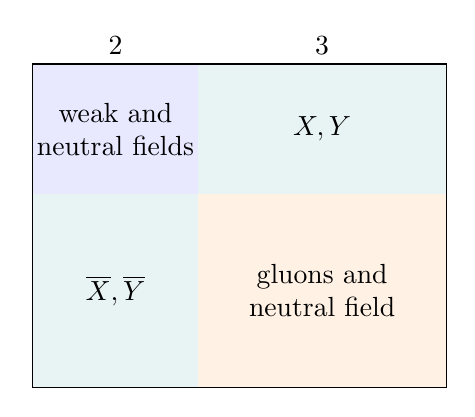
\begin{tikzpicture}[x=1.05cm,y=0.82cm]
  \draw[thick] (0,0) rectangle (5,5);
  \draw[thick] (2,0) -- (2,5);
  \draw[thick] (0,3) -- (5,3);
  \fill[blue!9] (0,3) rectangle (2,5);
  \fill[orange!10] (2,0) rectangle (5,3);
  \fill[teal!9] (2,3) rectangle (5,5);
  \fill[teal!9] (0,0) rectangle (2,3);
  \node[align=center] at (1,4) {weak and\\neutral fields};
  \node[align=center] at (3.5,1.5) {gluons and\\neutral field};
  \node[align=center] at (3.5,4) {\(X,Y\)};
  \node[align=center] at (1,1.5) {\(\overline X,\overline Y\)};
  \node[above] at (1,5) {\(2\)};
  \node[above] at (3.5,5) {\(3\)};
\end{tikzpicture}
\caption{Cấu trúc khối \(2\oplus3\) của trường chuẩn \(SU(5)\). Các khối ngoài đường chéo nối các lepton với các trường mang màu.}
\label{fig:l10-gauge-blocks}
\end{figure}

Với \(Q=T_3+Y\), doublet yếu mang màu trong phương trình~\eqref{eq:l10-adjoint-sm} có các điện tích \(-\tfrac13\) và \(-\tfrac43\); liên hợp của nó có \(+\tfrac13\) và \(+\tfrac43\). Bài giảng gọi các hạt này là \(X\) và \(Y\) nhưng nói rõ là không ấn định tên nào ứng với điện tích nào. Điều bất biến là kiểu chuyển tiếp và điện tích.

\begin{classroomqa}
\audiencequestion{Có ba phiên bản của mỗi boson chuẩn mới \(X\) hay \(Y\) không? \lecturetimestamp{00:41:28}}
\lecturerresponse{Có. Một chuyển tiếp nối một thành phần quark mang màu với một thành phần lepton không màu, nên boson trao đổi phải mang phần màu còn thiếu. Các trường \(X/Y\) tạo thành các triplet màu và có thể phát ra hoặc hấp thụ gluon.}
\end{classroomqa}

Các hạt mang màu không được quan sát như những trạng thái tiệm cận cô lập. Các boson chuẩn mới phải phân rã hoặc hadron hóa thành các tổ hợp trung hòa màu, đúng như quark vẫn làm.

\section{Vì sao đa bội chứa các phản quark down}

Các phần sinh của \(SU(N)\) là các ma trận Hermite không vết. Để thấy mối liên hệ với từ đặc biệt, hãy viết một phần tử nhóm vô cùng bé dưới dạng
\begin{equation}
U(\epsilon)=e^{i\epsilon T}.
\end{equation}
Tính unita cho \(T^\dagger=T\), còn
\begin{equation}
1=\det U=e^{i\epsilon\operatorname{tr}T}
\end{equation}
với mọi \(\epsilon\) kéo theo
\begin{equation}
\operatorname{tr}T=0.
\label{eq:l10-traceless-generator}
\end{equation}

Điện tích điện là một tổ hợp tuyến tính của các phần sinh. Trên cột vật chất trong phương trình~\eqref{eq:l10-fivebar}, nó tác dụng như
\begin{equation}
Q_{\overline5}
=
\operatorname{diag}
\left(0,-1,\frac13,\frac13,\frac13\right),
\qquad
\operatorname{tr}Q_{\overline5}=0.
\label{eq:l10-charge-fivebar}
\end{equation}
Do đó
\begin{equation}
0-1+3\left(\frac13\right)=0.
\end{equation}
Nếu thay các trường phản-down bằng các trường down thì thay vào đó sẽ có
\begin{equation}
0-1+3\left(-\frac13\right)=-2,
\end{equation}
mà không thể là vết của một phần sinh \(SU(5)\). Vì vậy, sự gán phản-down có vẻ lạ ấy thực ra bị áp đặt bởi cấu trúc nhóm.

\section{Mười fermion còn lại}

Mười trường còn lại xuất hiện từ một tensor phản đối xứng hai chỉ số. Theo quy ước chuẩn, đây là phần phản đối xứng của
\begin{equation}
\mathbf5\otimes\mathbf5
=\mathbf{15}_S\oplus\mathbf{10}_A.
\label{eq:l10-five-five}
\end{equation}
Bài giảng xây dựng nó bằng cách tạm thời viết các số lượng tử liên hợp
\begin{equation}
\chi=
\begin{pmatrix}
\nu^c\\
e^c\\
d_r\\
d_g\\
d_b
\end{pmatrix}.
\label{eq:l10-aux-five}
\end{equation}
Đây là một thủ pháp ghi sổ để lấy tích tensor các biểu diễn, chứ không phải là khẳng định rằng tồn tại một ngũ bội vật lý thứ hai gồm các hạt hợp thành.

Cho
\begin{equation}
\Psi^{ij}=-\Psi^{ji},
\qquad
i,j=1,\ldots,5.
\label{eq:l10-antisym-ten}
\end{equation}
Mọi phần tử trên đường chéo đều bằng không, và tam giác dưới được xác định bởi tam giác trên. Do đó
\begin{equation}
\dim\mathbf{10}
=\binom52
=\frac{5\cdot4}{2}
=10.
\label{eq:l10-ten-count}
\end{equation}

Điện tích của một phần tử là tổng các điện tích của hàng và cột trong Phương trình~\eqref{eq:l10-aux-five}. Điều này lập tức cho \(e^c\) ở ô yếu--yếu, các quark down và up trong các khối yếu--màu, và các trường phản-quark up trong khối màu--màu.

\begin{classroomqa}
\audiencequestion{Khi ghép các nhãn positron và quark down, phần tử thu được có phải là một boson \(X\) không? \lecturetimestamp{00:53:08}}
\lecturerresponse{Không. Ở giai đoạn này ta đang xây dựng biểu diễn fermion, không phải biểu diễn adjoint của boson chuẩn. Các điện tích cộng thành \(1-\tfrac13=\tfrac23\), nên phần tử ấy có các số lượng tử của một quark up.}
\end{classroomqa}

Một lựa chọn nhất quán cho các dấu màu là
\begin{equation}
\Psi^{ij}=
\begin{pmatrix}
0 & e^c & d_r & d_g & d_b\\
-e^c & 0 & u_r & u_g & u_b\\
-d_r & -u_r & 0 & u_b^c & -u_g^c\\
-d_g & -u_g & -u_b^c & 0 & u_r^c\\
-d_b & -u_b & u_g^c & -u_r^c & 0
\end{pmatrix}.
\label{eq:l10-ten-matrix}
\end{equation}
Thay đổi pha của các trường sẽ làm đổi một số dấu được viết ra, nhưng không làm đổi biểu diễn hay nội dung hạt.

\begin{figure}[htbp]
\centering
\includegraphics[width=0.83\textwidth]{lecture_10_figure_05.png}
\lectureframe{00:59:17.500}
\caption{Ma trận vật chất phản đối xứng \(2\oplus3\) hiển thị trọn vẹn sau khi các phần tử và nhãn màu đã được kiểm tra trên lớp.}
\label{fig:l10-ten-board}
\end{figure}

\begin{classroomqa}
\audiencequestion{Biểu diễn mười chiều có nhất thiết phải được viết dưới dạng ma trận không, hay có thể viết thành một cột? \lecturetimestamp{00:56:24}}
\lecturerresponse{Cả hai đều được. Có thể liệt kê 10 thành phần độc lập trong một cột, nhưng ma trận phản đối xứng \(5\times5\) cho thấy \(SU(5)\) tác dụng lên hai chỉ số của nó như thế nào, nên vì vậy giàu thông tin hơn nhiều.}
\end{classroomqa}

\begin{classroomqa}
\audiencequestion{Trong khối màu--màu, phần tử được ghi là \(u\) có thực ra phải là một trường phản-up không? \lecturetimestamp{00:57:51}}
\lecturerresponse{Đúng. Nhãn trên bảng được sửa thành \(u^c\), một trường phản-quark up tay trái. Hai điện tích cơ sở kiểu down cộng lại thành \(-\tfrac23\), đó là điện tích của một phản-quark up.}
\end{classroomqa}

\begin{classroomqa}
\audiencequestion{Các màu đã bị lược bỏ khỏi một số phần tử ma trận. Chúng vẫn được bảo toàn chứ? \lecturetimestamp{00:58:05}}
\lecturerresponse{Có. Ba vị trí màu là đỏ, lục và lam. Các nhãn chỉ bị lược bớt để giảm sự rối mắt.}
\end{classroomqa}

Một cặp phản đối xứng của hai biểu diễn cơ bản màu biến đổi như một phản-màu:
\begin{equation}
\wedge^2\mathbf3\simeq\overline{\mathbf3},
\qquad
(rg,rb,gb)\sim(\overline b,-\overline g,\overline r).
\label{eq:l10-anticolor}
\end{equation}
Đó là lý do vì sao ba phần tử độc lập trong khối màu--màu tạo thành đúng bộ ba màu của phản-up.

Một thế hệ nay đã được tổ chức thành
\begin{equation}
\overline{\mathbf5}\oplus\mathbf{10}.
\label{eq:l10-family}
\end{equation}
Điều đáng chú ý là \(u_L\) và \(u^c_L\) cùng xuất hiện trong một đa bội bất khả quy, trong khi \(d_L\) và \(d^c_L\), hoặc \(e_L\) và \(e^c_L\), lại nằm trong các đa bội khác nhau.

\begin{classroomqa}
\audiencequestion{Nếu các phép biến đổi chuẩn chỉ tác dụng trong từng biểu diễn, thì làm sao một khối lượng có thể nối các trường nằm trong 5-bar và 10? \lecturetimestamp{01:00:40}}
\lecturerresponse{Các boson chuẩn không quay một biểu diễn vật chất bất khả quy này thành biểu diễn kia. Các trường Higgs và các liên kết Yukawa có thể nối các biểu diễn khác nhau đồng thời tạo thành một tương tác bất biến tổng thể theo \(SU(5)\); sau khi trường Higgs nhận giá trị kỳ vọng, các tương tác ấy sinh ra khối lượng.}
\end{classroomqa}

\section{Các boson chuẩn tác dụng như những phép dịch chuyển}

Sau khi biểu diễn đã được lắp ghép xong, tác dụng của một boson chuẩn có thể được đọc như một phép dịch chuyển giữa các phần tử của nó. Một boson trung hòa có thể giữ nguyên một nhãn, một boson yếu dịch chuyển giữa các ô yếu, một gluon dịch chuyển giữa các ô màu, và một boson \(X/Y\) dịch chuyển giữa các ô yếu và màu. Các boson chuẩn mang điện có phản hạt, nên mỗi phép dịch chuyển đều có một quá trình ngược lại.

Đối với tensor phản đối xứng, một phép biến đổi vô cùng bé tác dụng lên mỗi chỉ số:
\begin{equation}
\delta\Psi^{ij}
=
i\epsilon
\left(
T^i{}_k\Psi^{kj}
+
T^j{}_k\Psi^{ik}
\right).
\label{eq:l10-two-index-action}
\end{equation}
Trong cách nhìn ma trận, hạng thứ nhất dịch theo phương dọc còn hạng thứ hai dịch theo phương ngang. Các nhãn thành phần dùng để dựng tensor chỉ là gợi nhớ; Phương trình~\eqref{eq:l10-two-index-action} mới là phát biểu lý thuyết nhóm chính xác.

Các phép dịch chuyển yếu biến \(d\) thành \(u\), tức quá trình ở mức quark đứng sau phân rã beta của neutron. Các phép dịch chuyển màu làm đổi đỏ, lục và lam mà không đổi hương. Các phép dịch chuyển ngoài đường chéo làm một điều mới:
\begin{equation}
\begin{aligned}
d^c&\longleftrightarrow e,
& d^c&\longleftrightarrow\nu,\\
d&\longleftrightarrow u^c,
& u&\longleftrightarrow e^c,
\end{aligned}
\label{eq:l10-leptoquark-shifts}
\end{equation}
với trường \(X/Y\) thích hợp mang độ chênh điện tích và màu.

\begin{classroomqa}
\audiencequestion{Các phép dịch chuyển giữa vị trí thứ tư và thứ năm biểu diễn điều gì, còn một phép dịch chuyển từ vị trí thứ nhất sang thứ tư thì sao? \lecturetimestamp{01:10:36}}
\lecturerresponse{Phép dịch chuyển thứ tư--thứ năm biến một màu thành màu khác và là một chuyển tiếp gluon. Phép dịch chuyển thứ nhất--thứ tư băng qua giữa khối yếu và khối màu, và là một trong các chuyển tiếp \(X/Y\) mới.}
\end{classroomqa}

\begin{classroomqa}
\audiencequestion{Có thể điền tường minh một phần tử của nửa dưới ma trận phản đối xứng không? \lecturetimestamp{01:11:23}}
\lecturerresponse{Có. Mỗi phần tử tam giác dưới là số âm của phần tử tam giác trên chuyển vị. Điền một phần tử sẽ làm quy tắc hiện rõ; điền hết tất cả chúng không thêm trạng thái mới nào.}
\end{classroomqa}

\section{Hệ quả nguy hiểm: phân rã proton}

Một boson \(X/Y\) có thể liên kết một quark với một lepton tại một đỉnh và hai trường kiểu quark tại một đỉnh khác. Ở các xung lượng nhỏ hơn nhiều so với khối lượng của nó, việc lấy tích phân loại bỏ boson nặng cho một tương tác bậc sáu theo thứ nguyên có dạng sơ đồ
\begin{equation}
\mathcal L_{\mathrm{eff}}
\sim
\frac{g_5^2}{M_X^2}\,(qq)(q\ell)
+\text{h.c.}
\label{eq:l10-effective-proton}
\end{equation}
Nó vi phạm riêng rẽ số baryon và số lepton, đồng thời bảo toàn các tổ hợp do tương tác chuẩn thống nhất quy định.

Trên bảng, ta theo dõi một quark down và một quark up qua quá trình trao đổi boson nặng. Quark down trở thành một positron, quark up trở thành một phản-quark up, và một quark up thứ hai không tham gia trực tiếp:
\begin{equation}
uud
\longrightarrow
e^++u\overline u.
\label{eq:l10-quark-decay}
\end{equation}
Trạng thái đầu là một proton. Cặp \(u\overline u\) có thể hadron hóa thành một pion trung hòa, cho
\begin{equation}
p\longrightarrow e^++\pi^0.
\label{eq:l10-proton-pion}
\end{equation}

\begin{figure}[htbp]
\centering
\includegraphics[width=0.82\textwidth]{lecture_10_figure_06.png}
\lectureframe{01:16:02.500}
\caption{Sơ đồ dựng trên bảng đã hoàn tất của sự trao đổi boson nặng bên trong một proton, với quark up không tham gia trực tiếp và kênh positron hiện rõ.}
\label{fig:l10-proton-board}
\end{figure}

Bài giảng cũng nhắc đến \(p\to e^++\gamma\), trong đó cặp quark--phản-quark hủy nhau theo điện từ. Kênh ấy chịu thêm một sự ức chế điện từ so với hadron hóa trực tiếp.

Khả năng này không phải là một chi tiết tô điểm tùy chọn của mô hình. Một khi một nhóm đơn chứa các bộ sinh nối quark với lepton, các quá trình vi phạm số baryon nói chung sẽ được kỳ vọng. Nếu chúng xảy ra trên các thang thời gian yếu hoặc điện từ thông thường, thì hạt nhân, hiđrô và vật chất vĩ mô sẽ không tồn tại.

\section{Vì sao proton sống lâu đến vậy?}

\begin{classroomqa}
\audiencequestion{Hằng số liên kết tạo ra một boson \(X\) có phải cũng là hằng số liên kết thống nhất được phần còn lại của nhóm dùng đến không? \lecturetimestamp{01:18:34}}
\lecturerresponse{Ở thang thống nhất thì đúng vậy. Một lý thuyết chuẩn \(SU(5)\) đơn có một hằng số liên kết chuẩn duy nhất là \(g_5\). Các hằng số liên kết mạnh, yếu và siêu điện tích ở năng lượng thấp khác nhau vì sau khi đối xứng thống nhất bị phá vỡ, chúng chạy khác nhau.}
\end{classroomqa}

Không thể chọn hằng số liên kết nhỏ một cách phi thực tế mà không từ bỏ cấu trúc thống nhất. Nguồn ức chế khả dĩ là propagator nặng:
\begin{equation}
\mathcal A
\sim
\frac{g_5^2}{M_X^2}.
\label{eq:l10-amplitude}
\end{equation}
Bình phương biên độ cho \(g_5^4/M_X^4\). Phân tích thứ nguyên và phần tử ma trận proton hoàn tất ước lượng suất phân rã:
\begin{equation}
\Gamma_p
\sim
C_{\mathrm{had}}\,
\frac{\alpha_5^2\,m_p^5}{M_X^4},
\qquad
\alpha_5=\frac{g_5^2}{4\pi},
\label{eq:l10-rate}
\end{equation}
trong đó \(C_{\mathrm{had}}\) chứa các hệ số nhóm, các hiệu ứng tái chuẩn hóa và phần tử ma trận hadron phi nhiễu loạn.

\editorialnote{Bài giảng tách riêng sự phụ thuộc thiết yếu vào \(g^4/M_X^4\) và lưu ý rằng các thừa số khối lượng proton đã bị lược bỏ. Phương trình~\eqref{eq:l10-rate} khôi phục thứ nguyên khối lượng cần thiết mà không ngụ ý một phép tính thời gian sống chính xác.}

\begin{classroomqa}
\audiencequestion{Liệu thừa số nhỏ \(g^4\), có lẽ cỡ \(10^{-8}\) trong ước lượng gần đúng trên lớp, đã đủ làm thời gian sống dài lên hay chưa? \lecturetimestamp{01:25:13}}
\lecturerresponse{Chưa. Nó có giúp, nhưng khoảng cách giữa một thời gian vi mô của tương tác mạnh và cận dưới thời gian sống của proton trải qua nhiều bậc độ lớn hơn thế rất nhiều. Lũy thừa bậc bốn của khối lượng nặng mới phải cung cấp sự ức chế quyết định.}
\end{classroomqa}

Nếu mọi khối lượng đều cỡ khối lượng proton, thì đơn vị thời gian tự nhiên sẽ xấp xỉ thời gian ánh sáng đi qua một proton:
\begin{equation}
t_p\sim\frac{1\ \mathrm{fm}}{c}\sim10^{-23}\ \mathrm{s}.
\label{eq:l10-proton-time}
\end{equation}
Chỉ riêng sự tồn tại của các proton nguyên thủy cũng đã cho thấy thời gian sống của chúng vượt quá tuổi của vũ trụ, nhưng các phép tìm kiếm trong phòng thí nghiệm còn đi xa hơn rất nhiều. Bài giảng so sánh ước lượng vi mô với giới hạn thực nghiệm được trích dẫn khi đó
\begin{equation}
\tau_p\gtrsim10^{33}\ \mathrm{yr}.
\label{eq:l10-lifetime-bound}
\end{equation}

Không cần phải theo dõi một proton đơn lẻ lâu đến thế. Nếu thời gian sống là \(10^{15}\) năm, thì một mẫu gồm \(10^{15}\) proton sẽ cho xấp xỉ một sự kiện mỗi năm. Tổng quát hơn, với \(N_p\) proton được quan sát trong thời gian \(T\), số phân rã kỳ vọng là
\begin{equation}
\langle n\rangle\simeq\frac{N_pT}{\tau_p}.
\label{eq:l10-event-count}
\end{equation}
Một detector chứa khoảng \(10^{33}\) proton là một bể lớn chứ không phải một vật thể thiên văn: bản thân số proton ấy có khối lượng cỡ \(10^6\) kilôgam. Theo dõi một mẫu như vậy biến một thời gian sống khổng lồ của từng proton thành một tốc độ sự kiện đo được hoặc một cận dưới mạnh hơn.

Kết hợp Phương trình~\eqref{eq:l10-rate} với ràng buộc về thời gian sống sẽ đẩy khối lượng boson chuẩn leptoquark lên cỡ
\begin{equation}
M_X\sim10^{15}\text{--}10^{16}\ \mathrm{GeV},
\label{eq:l10-mx}
\end{equation}
với \(10^{16}\,\mathrm{GeV}\) được dùng trong bài giảng như thang an toàn dễ nhớ. Điều này thấp hơn thang Planck vài bậc độ lớn và vì vậy không tự động mâu thuẫn với lý thuyết trường lượng tử.

\section{\texorpdfstring{\(SU(5)\)}{SU(5)} bị phá vỡ và thang thống nhất}

Các trường \(X/Y\) cùng nằm trong một đa bội adjoint của \(SU(5)\) với các trường chuẩn của Mô hình Chuẩn. Một đối xứng chuẩn chính xác chưa bị phá vỡ sẽ không cho phép một số thành phần có khối lượng gần \(10^{16}\,\mathrm{GeV}\) trong khi photon và các gluon vẫn không khối lượng. Vì thế đối xứng ấy tất yếu phải bị phá vỡ tự phát.

\begin{classroomqa}
\audiencequestion{Nếu đối xứng \(SU(5)\) không bị phá vỡ, liệu tất cả các boson chuẩn của nó có đều không khối lượng không? \lecturetimestamp{01:29:37}}
\lecturerresponse{Có, trong lý thuyết chuẩn đang được bàn đến. Bất biến chuẩn cấm một khối lượng chung đưa vào tường minh. Một cơ chế Higgs có thể cho khối lượng đối với các boson chuẩn gắn với những bộ sinh bị phá vỡ, đồng thời để các trường chuẩn của phân nhóm không bị phá vỡ vẫn không khối lượng.}
\end{classroomqa}

Cơ chế Higgs điện yếu đã minh họa khuôn mẫu này: nó phân biệt photon với \(W^\pm\) và \(Z\). Thống nhất lớn đòi hỏi một tham số trật tự riêng ở thang cao, tham số này phân biệt khối yếu \(2\) với khối màu \(3\) và làm cho các trường \(X/Y\) ngoài đường chéo trở nên cực nặng.

So với \(10^{16}\,\mathrm{GeV}\), ngay cả khối lượng boson yếu \(100\,\mathrm{GeV}\) cũng không đáng kể. Ở đủ cao trên ngưỡng nặng, có thể bỏ qua mọi khối lượng boson chuẩn và toàn bộ đối xứng \(SU(5)\) trở thành một gần đúng tốt. Đó là ý nghĩa của một thang thống nhất: không phải là thế giới năng lượng thấp hiển nhiên có \(SU(5)\), mà là các quá trình đủ năng lượng trở nên không nhạy với các sự phân tách khối lượng do phá vỡ đối xứng.

\section{Sự chạy của các hằng số liên kết}

Các hằng số liên kết chuẩn phụ thuộc lôgarit vào thang năng lượng. Định nghĩa
\begin{equation}
\alpha_i(\mu)=\frac{g_i^2(\mu)}{4\pi},
\end{equation}
thì sự tiến hóa ở một vòng có dạng
\begin{equation}
\alpha_i^{-1}(\mu)
=
\alpha_i^{-1}(\mu_0)
-\frac{b_i}{2\pi}
\ln\!\left(\frac{\mu}{\mu_0}\right).
\label{eq:l10-running}
\end{equation}
Các hệ số \(b_i\) phụ thuộc vào nhóm chuẩn và vào mọi hạt đủ nhẹ để chạy trong các vòng lượng tử liên quan.

\editorialnote{Để so sánh siêu điện tích với các hằng số liên kết không Abel bên trong \(SU(5)\), phải gán cho \(g_1\) chuẩn hóa thống nhất lớn theo quy ước. Đây là nguồn gốc của các hệ số số học lý thuyết nhóm được nhắc đến trong bài giảng.}

Ở các năng lượng trong phòng thí nghiệm, nghịch đảo của ba hằng số liên kết là khác nhau. Theo thứ tự định tính trong bài giảng, \(1/\alpha_1\) là lớn nhất vì liên kết siêu tích là yếu nhất, \(1/\alpha_2\) đứng kế tiếp, và \(1/\alpha_3\) là nhỏ nhất vì tương tác mạnh là mạnh nhất. Các đường cong ở những năng lượng không thể tiếp cận không được đo trực tiếp. Chúng được tính từ các giá trị năng lượng thấp quan sát được, phổ hạt, và các giản đồ vòng xác định các hàm beta. Với thành phần hạt của Mô hình Chuẩn, khi vẽ theo \(\log\mu\), chúng trở thành gần như các đường thẳng.

\begin{figure}[htbp]
\centering
\includegraphics[width=0.74\textwidth]{lecture_10_figure_07.png}
\lectureframe{01:36:32.500}
\caption{Đồ thị trên bảng biểu diễn các nghịch đảo của các hằng số liên kết chuẩn tiến lại gần nhau gần \(10^{16}\,\mathrm{GeV}\). Vùng được khoanh tròn đánh dấu chỗ chúng gặp nhau không hoàn toàn.}
\label{fig:l10-running-board}
\end{figure}

Dưới ngưỡng thống nhất, đối xứng bị phá vỡ, phổ nhẹ không lấp đầy các đa tuyến \(SU(5)\) đầy đủ và suy biến, và ba hệ số của hàm beta khác nhau. Do đó các hằng số liên kết chạy với tốc độ khác nhau. Ở thang năng lượng cao, người ta hỏi liệu chúng có đạt tới một giá trị chung hay không:
\begin{equation}
\alpha_1(M_{\mathrm{GUT}})
\stackrel{?}{=}
\alpha_2(M_{\mathrm{GUT}})
\stackrel{?}{=}
\alpha_3(M_{\mathrm{GUT}}).
\label{eq:l10-unification-condition}
\end{equation}

Chỉ với phổ Mô hình Chuẩn không siêu đối xứng, các đường tiến lại gần nhau quanh \(10^{15}\)--\(10^{16}\,\mathrm{GeV}\) nhưng vẫn lệch nhau một lượng đáng kể; bài giảng mô tả mức độ phù hợp là xấp xỉ 15 phần trăm. Sự trùng hợp quan trọng là đây cũng là thang năng lượng mà tính ổn định của proton đòi hỏi.

\section{Một câu hỏi cuối cùng về neutron}

\begin{classroomqa}
\audiencequestion{Nếu quark up không tham gia trong giản đồ phân rã proton được thay bằng một quark down, thì điều đó có mô tả sự phân rã neutron không, và boson \(X\) có liên quan không? \lecturetimestamp{01:36:40}}
\lecturerresponse{Nó sẽ xác định một kênh neutron của thống nhất lớn như \(n\to e^++\pi^-\), nhưng đó không phải là sự phân rã quen thuộc của một neutron tự do. Phân rã beta thông thường của neutron là \(n\to p+e^-+\overline\nu_e\) và diễn ra thông qua tương tác yếu. Nếu thứ tự khối lượng proton--neutron bị đảo ngược, thì trạng thái bền đối với phân rã beta cũng sẽ đảo ngược theo, còn kênh thống nhất lớn chậm hơn nhiều kia vẫn có thể tồn tại.}
\end{classroomqa}

Sự phân biệt này tách động học khỏi tương tác mới. Nuclôn nào phân rã beta phụ thuộc vào độ chênh khối lượng proton--neutron; sự vi phạm số baryon do trao đổi \(X/Y\) là một cơ chế riêng biệt, bị ức chế cực kỳ mạnh.

\section{Siêu đối xứng và bức tranh rộng hơn}

Việc thêm phổ các siêu đối tác làm thay đổi các hệ số của hàm beta trong phương trình~\eqref{eq:l10-running}. Theo trình bày của bài giảng, khi đó ba hằng số liên kết được ngoại suy gặp nhau với độ chính xác khoảng 1 phần trăm. Điều này không chứng minh siêu đối xứng hay thống nhất lớn, nhưng đó là lý do thực nghiệm khiến hai ý tưởng này thường được thảo luận cùng nhau.

Các đa tuyến vật chất còn có thể được thống nhất thêm nữa. Theo
\begin{equation}
SO(10)\supset SU(5),
\end{equation}
một biểu diễn spinor phân rã thành
\begin{equation}
\mathbf{16}
\longrightarrow
\mathbf{10}\oplus\overline{\mathbf5}\oplus\mathbf1.
\label{eq:l10-so10}
\end{equation}
Biểu diễn singlet được đồng nhất một cách tự nhiên với một phản neutrino tay trái, hay tương đương là liên hợp điện tích của một neutrino tay phải. Vì vậy, cả 16 trường của một họ mở rộng đều nằm gọn trong một đa tuyến \(SO(10)\) bất khả quy.

Các thí nghiệm phân rã proton tiếp tục kiểm tra ý tưởng này bằng cách nâng cận dưới của thời gian sống lên khi không quan sát thấy sự kiện nào. Các mô hình thống nhất lớn siêu đối xứng không cho một thời gian sống proton phổ quát duy nhất: các trường nặng bổ sung và các toán tử phụ thuộc vào siêu đối tác có thể làm thay đổi kênh trội và tốc độ trên một khoảng rất rộng.

\editorialnote{Trong thống nhất lớn siêu đối xứng, sự trao đổi Higgs bộ ba màu có thể sinh ra các toán tử vi phạm số baryon bậc năm, bên cạnh toán tử boson chuẩn bậc sáu được thảo luận ở đây. Các hệ số của chúng phụ thuộc mạnh vào phổ nặng, cấu trúc hương vị và khối lượng các siêu đối tác, điều này giải thích lời lưu ý trong bài giảng rằng chỉ riêng siêu đối xứng không dẫn đến một thời gian sống duy nhất.}

Bài học lâu dài ở đây là một thế căng thẳng chứ không phải một kết luận dứt khoát. Lý thuyết nhóm đặt quark và lepton vào cùng một khuôn khổ với độ gọn đáng kinh ngạc, các hằng số liên kết chạy gợi ý một thang năng lượng cao chung, và siêu đối xứng làm sắc nét thêm gợi ý định lượng đó. Cùng một cấu trúc ấy cũng dự đoán sự chuyển hóa nguy hiểm của quark thành lepton. Vì vậy, bất kỳ phiên bản thành công nào cũng phải giữ được sự tao nhã ấy đồng thời giữ cho proton ổn định trong một thời gian gần như không thể tưởng tượng nổi. Theo tinh thần kết thúc của bài giảng: cầu mong mọi proton của chúng ta đều vẫn ổn định.
